\documentclass[12pt,a4paper]{article}


\newcommand{\AppName}{Maxwell Bloch Studio}
\newcommand{\AppVersion}{10.0.6}
  % written from pyproject.toml by tools/build_docs.sh
\newcommand{\AppAuthor}{Vahid Anari}
\newcommand{\AppEmail}{vahid.anari8@gmail.com}
\newcommand{\DocName}{Equations Reference}
\usepackage{style}

% ── Convenience macros ────────────────────────────────────────────────────────
\newcommand{\T}{T_0}
\newcommand{\mb}{Maxwell--Bloch}
\newcommand{\pderiv}[2]{\dfrac{\partial #1}{\partial #2}}

% ══════════════════════════════════════════════════════════════════════════════
\begin{document}

% ── Title page ────────────────────────────────────────────────────────────────
\begin{titlepage}
  \centering
  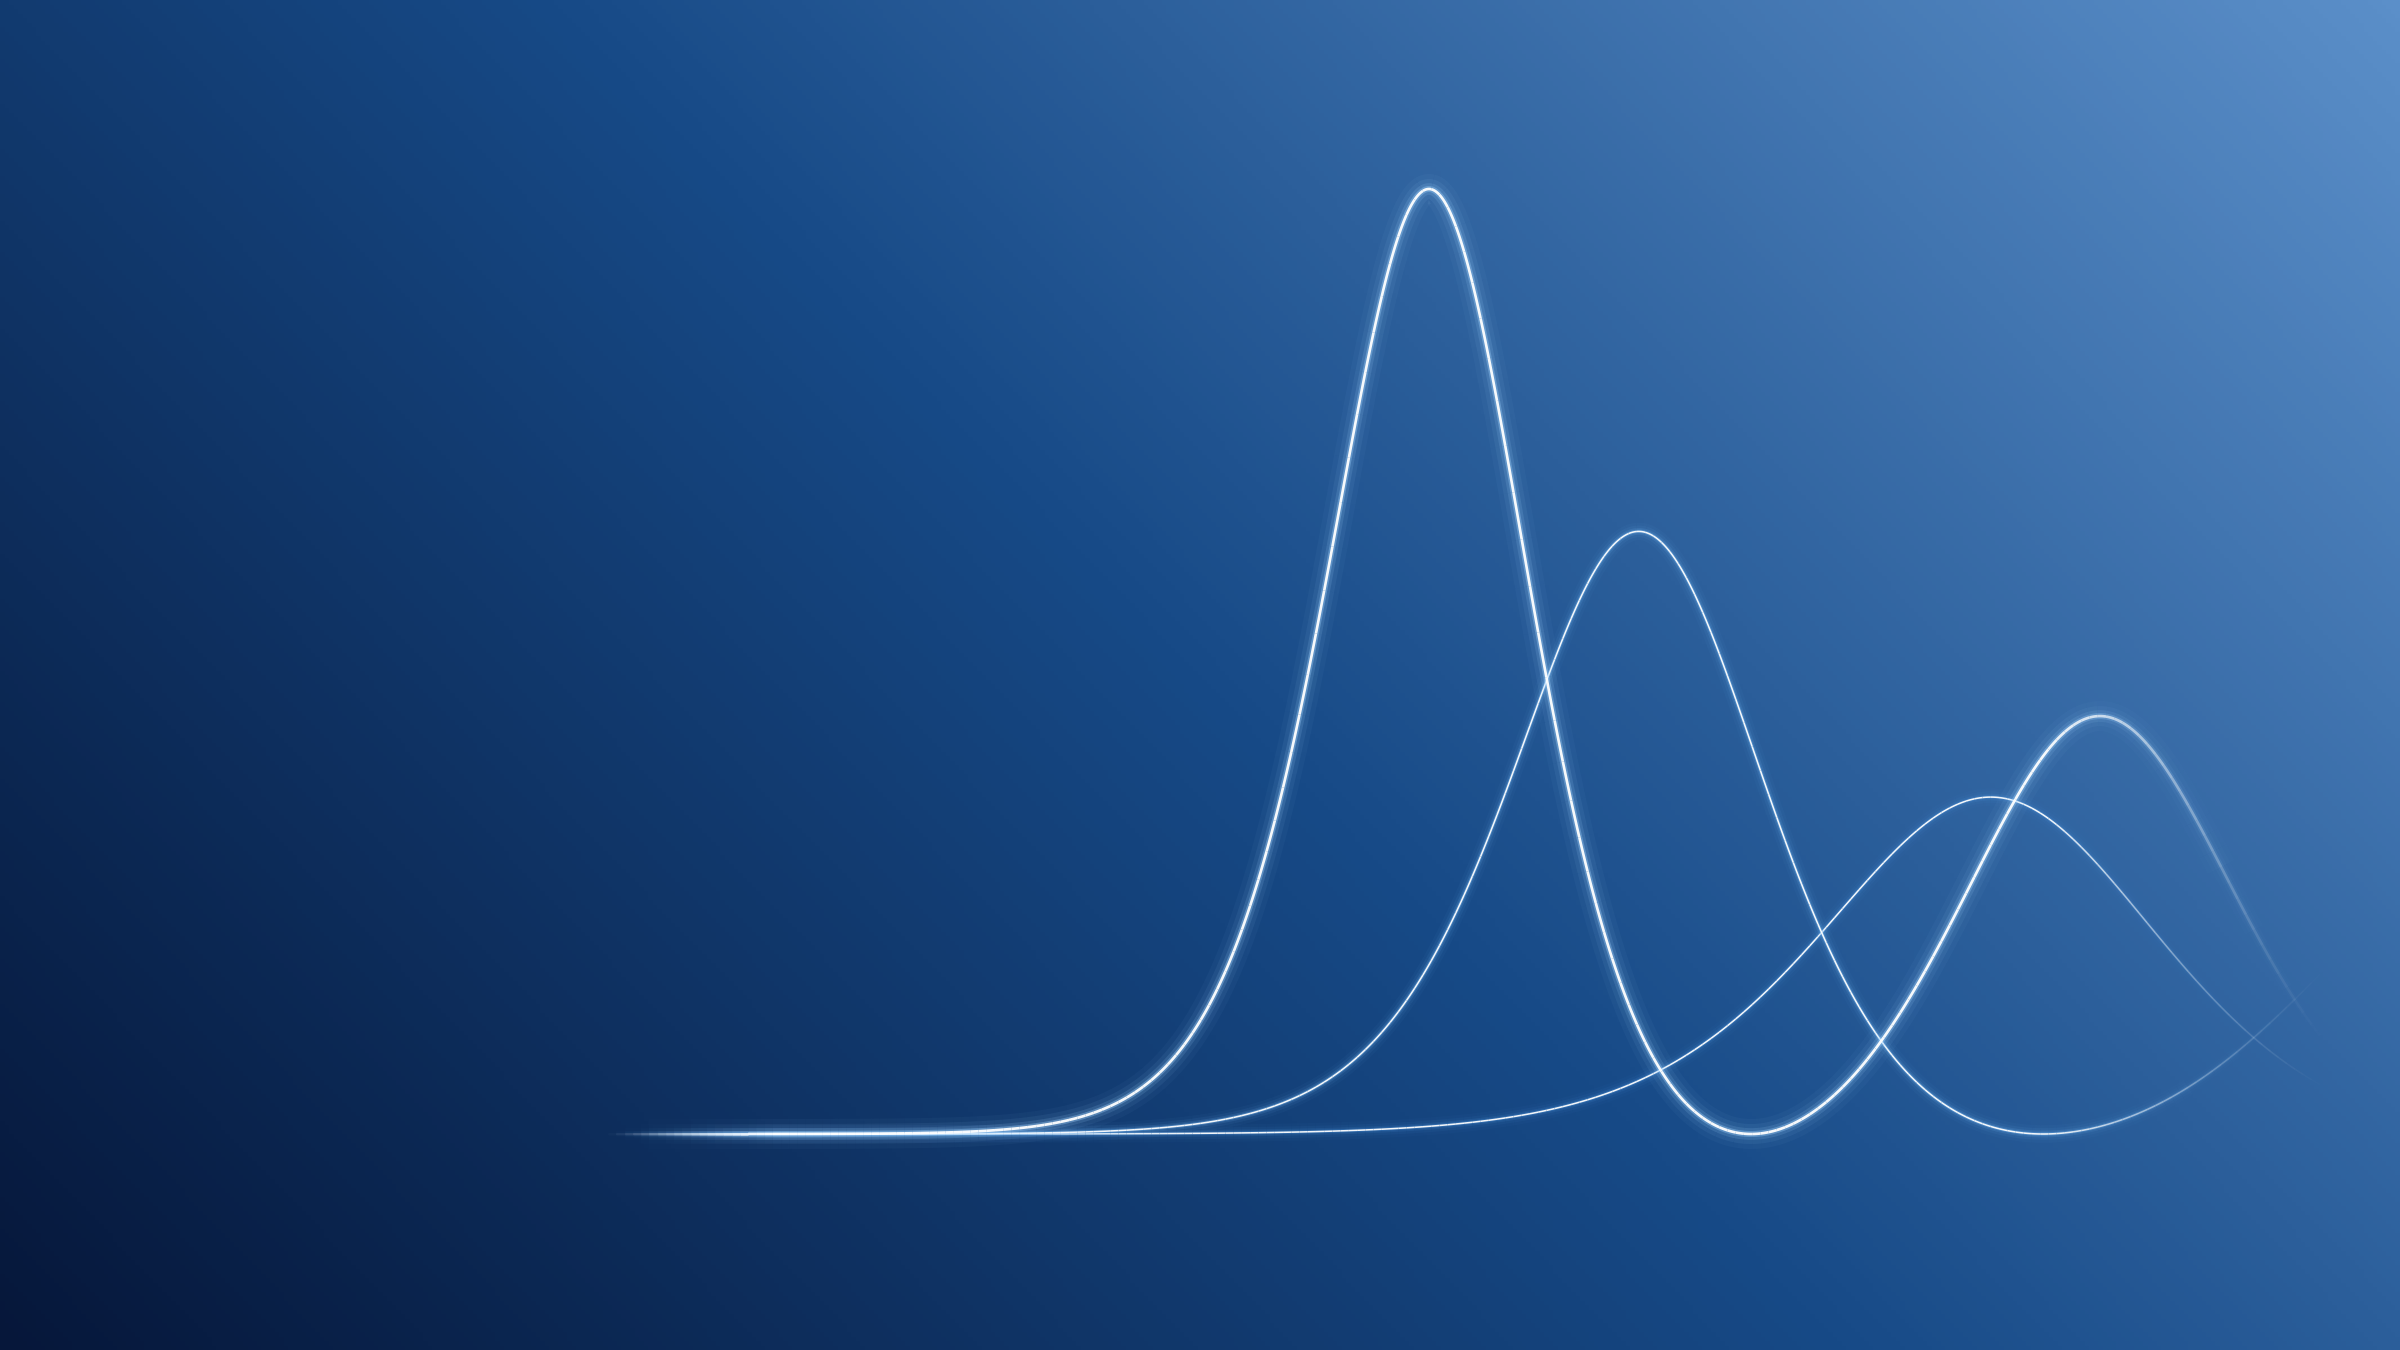
\includegraphics[width=\textwidth,trim=180 0 0 0,clip]{figures/splash.png}\\[2cm]
  {\Huge\bfseries\color{accent} \AppName}\\[0.5em]
  {\large \DocName}\\[0.3em]
  {\normalsize Version \AppVersion}\\[3cm]
  {\large \AppAuthor}\\[0.4em]
  \href{mailto:\AppEmail}{\texttt{\AppEmail}}\\[3cm]
  \vfill
  {\small\color{gray}
  This document derives the dimensionless \mb{} equations used by the solver,
  starting from the general two-level Hamiltonian and proceeding through the
  rotating-wave and slowly-varying-envelope approximations to the final
  dimensionless system.}
\end{titlepage}

\tableofcontents
\newpage

% ══════════════════════════════════════════════════════════════════════════════
\section{Hamiltonian}

Let $|2\rangle$ denote the upper state and $|1\rangle$ the lower state of a
two-level system with transition frequency $\omega_0$. The free Hamiltonian is
\begin{equation}
  \hat{H}_0 = \frac{\hbar\omega_0}{2}\hat{\sigma}_z,
  \qquad
  \hat{\sigma}_z = |2\rangle\langle 2| - |1\rangle\langle 1|,
\end{equation}
with raising and lowering operators
\begin{equation}
  \hat{\sigma}_+ = |2\rangle\langle 1|,
  \qquad
  \hat{\sigma}_- = |1\rangle\langle 2|.
\end{equation}

The electric dipole operator is written in terms of the transition matrix
elements $\bm{d}_{21} = \langle 2|\hat{\bm{d}}|1\rangle$ and
$\bm{d}_{12} = \bm{d}_{21}^*$ as
\begin{equation}
  \hat{\bm{d}} = \bm{d}_{21}\,\hat{\sigma}_+ + \bm{d}_{12}\,\hat{\sigma}_-.
\end{equation}

Writing the electric field along polarization unit vector $\hat{\bm{e}}$ as
$\bm{E} = E\hat{\bm{e}}$ and defining the scalar transition matrix element
\begin{equation}
  d = \bm{d}_{21}\cdot\hat{\bm{e}},
\end{equation}
the interaction Hamiltonian takes the form
\begin{equation}
  \hat{H}_{\mathrm{int}}
  = -\hat{\bm{d}}\cdot\bm{E}
  = -\bigl(d\,\hat{\sigma}_+ + d^*\hat{\sigma}_-\bigr)E.
\end{equation}

The total Hamiltonian is $\hat{H} = \hat{H}_0 + \hat{H}_{\mathrm{int}}$.

% ══════════════════════════════════════════════════════════════════════════════
\section{Density-Matrix Equations of Motion}

The state of the medium is described by the density operator
\begin{equation}
  \hat{\rho} = \sum_{m,n\,\in\,\{1,2\}} \rho_{mn}\,|m\rangle\langle n|,
\end{equation}
with population inversion
\begin{equation}
  w = \rho_{22} - \rho_{11}, \qquad \rho_{21} = \rho_{12}^*.
\end{equation}

From the Liouville--von Neumann equation
$i\hbar\dot{\hat{\rho}} = [\hat{H},\hat{\rho}]$,
the matrix element $\langle 1|\,[\hat{H},\hat{\rho}]\,|2\rangle$ gives
\begin{align}
  i\hbar\dot{\rho}_{12}
  &= \langle 1|[\hat{H},\hat{\rho}]|2\rangle \notag\\
  &= -\hbar\omega_0\rho_{12} - d^*E\,(\rho_{22}-\rho_{11}),
\end{align}
giving
\begin{equation}
  \dot{\rho}_{12} = i\omega_0\rho_{12} + \frac{id^*}{\hbar}\,E\,w.
  \label{eq:rho12full}
\end{equation}

Since $\rho_{21} = \rho_{12}^*$, the complex conjugate gives immediately
\begin{equation}
  \dot{\rho}_{21} = -i\omega_0\rho_{21} - \frac{id}{\hbar}\,E\,w.
  \label{eq:rho21full}
\end{equation}

For the inversion, taking
$\langle 2|[\hat{H},\hat{\rho}]|2\rangle - \langle 1|[\hat{H},\hat{\rho}]|1\rangle$:
\begin{equation}
  i\hbar\dot{w} = 2\bigl(d^*E\,\rho_{21} - dE\,\rho_{12}\bigr),
\end{equation}
so that
\begin{equation}
  \dot{w} = \frac{2i}{\hbar}\bigl(dE\,\rho_{12} - d^*E\,\rho_{21}\bigr).
  \label{eq:wfull}
\end{equation}

% ══════════════════════════════════════════════════════════════════════════════
\section{Maxwell Wave Equations}

\subsection{Maxwell's equations}

In a medium with no free charges or currents, Maxwell's equations are
\begin{align}
  \nabla \cdot \mathbf{D} &= 0, \\
  \nabla \cdot \mathbf{B} &= 0, \\
  \nabla \times \mathbf{E} &= -\pderiv{\mathbf{B}}{t}, \\
  \nabla \times \mathbf{H} &= \pderiv{\mathbf{D}}{t},
\end{align}
with constitutive relations
\begin{equation}
  \mathbf{D} = \epsilon_0\mathbf{E} + \mathbf{P},
  \qquad
  \mathbf{B} = \mu_0\bigl(\mathbf{H} + \mathbf{M}\bigr).
\end{equation}

\subsection{General wave equations}

Taking the curl of the curl equations and using the constitutive relations
gives the general wave equations for $\mathbf{E}$ and $\mathbf{B}$:
\begin{equation}
  \nabla^2\mathbf{E} - \mu_0\epsilon_0\pderiv{^2\mathbf{E}}{t^2}
  = \mu_0\pderiv{^2\mathbf{P}}{t^2}
  + \mu_0\nabla\times\pderiv{\mathbf{M}}{t},
  \label{eq:waveE}
\end{equation}
\begin{equation}
  \nabla^2\mathbf{B} - \mu_0\epsilon_0\pderiv{^2\mathbf{B}}{t^2}
  = -\mu_0\nabla\times\!\left(\pderiv{\mathbf{P}}{t}
  + \nabla\times\mathbf{M}\right).
  \label{eq:waveB}
\end{equation}

\subsection{Reduction to one dimension}

We consider a plane wave propagating along $z$ with fields transverse to $z$.
For the \textbf{electric-dipole} case the medium has no magnetization
($\mathbf{M}=0$), so the curl term in Eq.~(\ref{eq:waveE}) vanishes and
the wave equation reduces to
\begin{equation}
  \pderiv{^2 E}{z^2} - \frac{1}{c^2}\pderiv{^2 E}{t^2}
  = \mu_0\pderiv{^2 P}{t^2}.
  \label{eq:wave1DE}
\end{equation}

The macroscopic polarization is related to the density operator through
\begin{equation}
  P = n_0\operatorname{Tr}(\hat{\rho}\,\hat{\bm{d}}\cdot\hat{\bm{e}})
    = n_0\bigl(\rho_{12}\,d + \rho_{21}\,d^*\bigr).
\end{equation}

% ══════════════════════════════════════════════════════════════════════════════
\section{Slowly Varying Envelope and Rotating-Wave Approximations}

We apply two standard approximations: the \textbf{slowly varying envelope
approximation} (SVEA) to the field, and the \textbf{rotating-wave
approximation} (RWA) to the atom--field coupling.

\subsection{Envelope decomposition}

The field and coherence $\rho_{21}$ are written as slowly varying envelopes
modulated by the carrier $e^{i(kz-\omega t)}$:
\begin{equation}
  E(z,t) = \tfrac{1}{2}A(z,t)\,e^{i(kz-\omega t)} + \mathrm{c.c.},
\end{equation}
\begin{equation}
  \rho_{21}(z,t) = \tfrac{1}{2}R(z,t)\,e^{i(kz-\omega t)},
\end{equation}
where $k = \omega/c$ is the carrier wave number, and $A$ and $R$ satisfy
\begin{equation}
  \left|\pderiv{A}{t}\right| \ll \omega|A|,
  \quad
  \left|\pderiv{A}{z}\right| \ll k|A|,
\end{equation}
and similarly for $R$. The factor of $\tfrac{1}{2}$ ensures that $A$ equals
the peak amplitude of the field.

\subsection{Equations of motion}

Substituting the envelope decomposition into Eq.~(\ref{eq:rho21full}),
collecting terms at the resonant frequency $e^{i(kz-\omega t)}$,
and dropping the fast counter-rotating terms (RWA). we define the detuning
\begin{equation}
  \Delta = \omega - \omega_0,
\end{equation}
the coherence equation becomes
\begin{equation}
  \dot{R} = i\Delta R - \frac{id}{\hbar}\,A\,w.
\end{equation}

Substituting into Eq.~(\ref{eq:wfull}) and keeping only the two resonant
products (one from each factor of the field and coherence):
\begin{equation}
  \dot{w} = \frac{i}{2\hbar}\bigl(dAR^* - d^*A^*R\bigr).
\end{equation}

Substituting into the wave equation~(\ref{eq:wave1DE}), dropping second-order
derivatives of $A$ (SVEA), and using $k = \omega/c$:
\begin{equation}
  \pderiv{A}{z} + \frac{1}{c}\pderiv{A}{t}
  = \frac{i\omega\,n_0 d^*}{2\epsilon_0 c}\,R.
\end{equation}

\subsection{Relaxation and pumping}

In practice the two-level medium is coupled to its environment, leading to
population relaxation on a timescale $T_1$ and dephasing on a timescale $T_2$.
These are added phenomenologically. A pump term $\Lambda_n$ drives the
inversion away from its equilibrium value $w_0$, and the coherence relaxes
toward its equilibrium value $R_0$. We also set the detuning $\Delta = 0$,
corresponding to exact resonance between the carrier and the atomic transition.
The full Maxwell--Bloch system is:
\begin{align}
  \pderiv{w}{t}
    &= \frac{i}{2\hbar}\bigl(dAR^* - d^*A^*R\bigr)
       - \frac{w - w_0}{T_1}
       + \Lambda_n,
  \label{eq:invSVEA}\\[4pt]
  \pderiv{R}{t}
    &= - \frac{id}{\hbar}\,A\,w - \frac{R - R_0}{T_2},
  \label{eq:cohSVEA}\\[4pt]
  \pderiv{A}{z} + \frac{1}{c}\pderiv{A}{t}
    &= \frac{i\omega\,n_0 d^*}{2\epsilon_0 c}\,R.
  \label{eq:fieldSVEA}
\end{align}

% ══════════════════════════════════════════════════════════════════════════════
\section{Retarded-Time Coordinates}

We move to a frame co-propagating with the field by introducing the retarded
time $\tau = t - z/c$, keeping $z$ as the propagation coordinate.
Under this transformation
\begin{equation}
  \frac{\partial}{\partial z}\bigg|_t
  = \frac{\partial}{\partial z}\bigg|_\tau
  - \frac{1}{c}\frac{\partial}{\partial \tau}\bigg|_z,
  \qquad
  \frac{\partial}{\partial t}\bigg|_z
  = \frac{\partial}{\partial \tau}\bigg|_z,
\end{equation}
so the operator $\partial_z|_t + c^{-1}\partial_t|_z$ reduces to
$\partial_z|_\tau$, and the field equation becomes a pure spatial
propagation equation. The full Maxwell--Bloch system in retarded-time
coordinates is:
\begin{align}
  \pderiv{w}{\tau}
    &= \frac{i}{2\hbar}\bigl(dAR^* - d^*A^*R\bigr)
       - \frac{w - w_0}{T_1}
       + \Lambda_n,
  \label{eq:invRet}\\[4pt]
  \pderiv{R}{\tau}
    &= - \frac{id}{\hbar}\,A\,w - \frac{R-R_0}{T_2},
  \label{eq:cohRet}\\[4pt]
  \pderiv{A}{z}
    &= \frac{i\omega\,n_0 d^*}{2\epsilon_0 c}\,R.
  \label{eq:fieldRet}
\end{align}

% ══════════════════════════════════════════════════════════════════════════════
\section{Dimensionless Form}

\subsection{Scaled variables}

The inversion $w$ and coherence $R$ are already dimensionless. We introduce
dimensionless forms of the remaining variables by normalising lengths to the
sample length $L$, times to the characteristic scale $\T$, and the field
amplitude to $\hbar/d\T$:
\begin{equation}
  z' = \frac{z}{L}, \qquad \tau' = \frac{\tau}{\T},
  \qquad T_1' = \frac{T_1}{\T}, \qquad T_2' = \frac{T_2}{\T},
  \qquad \Lambda_n' = \T\Lambda_n.
\end{equation}

To absorb the imaginary unit in the field equation we define the
dimensionless field amplitude
\begin{equation}
  A' = \frac{A}{A_0},
  \label{eq:Adef}
\end{equation}
where the field amplitude scale is
\begin{equation}
  A_0 = -i\frac{\hbar}{d\,\T}.
  \label{eq:A0}
\end{equation}

\subsection{Cooperation time $T_R$}

Substituting Eqs.~(\ref{eq:Adef})--(\ref{eq:A0}) into
Eq.~(\ref{eq:fieldRet}):
\begin{equation}
  \pderiv{A'}{z'} = -\eta\,R,
\end{equation}
where
\begin{equation}
  \eta = \frac{\T}{T_R},
  \label{eq:eta}
\end{equation}
and the \textbf{cooperation time} is defined as
\begin{equation}
  \boxed{T_R = \frac{2\epsilon_0 c\hbar}{\omega\,|d|^2\,n_0\,L}.}
  \label{eq:TR}
\end{equation}

\subsection{Final dimensionless equations}

Substituting Eq.~(\ref{eq:Adef}) into
Eqs.~(\ref{eq:invRet})--(\ref{eq:fieldRet}) and expressing all times in
units of $\T$:

\begin{resultbox}
\begin{align}
  \pderiv{w}{\tau'}
    &= \operatorname{Re}(A'R^*)
       - \frac{w - w_0}{T_1'}
       + \Lambda_n',
  \label{eq:dimw}\\[8pt]
  \pderiv{R}{\tau'}
    &= -A'\,w - \frac{R-R_0}{T_2'},
  \label{eq:dimR}\\[8pt]
  \pderiv{A'}{z'}
    &= -\eta R.
  \label{eq:dimA}
\end{align}
\end{resultbox}

\begin{notebox}
  No explicit $\hbar$, $d$, or $\T$ appear in
  Eqs.~(\ref{eq:dimw})--(\ref{eq:dimA}).
  All microscopic parameters are absorbed into $\eta$
  and the dimensionless field amplitude $A'$.
\end{notebox}

\subsection{Symbol table}
\begin{center}
\begin{tabular}{@{}llcc@{}}
  \toprule
  Symbol & Meaning & Range & Units \\
  \midrule
  $A_0 = -i\hbar/d\T$        & Field amplitude scale                            & $\mathbb{C}$   & (V/m) \\
  $A' = A/A_0$               & Dimensionless field envelope                     & $\mathbb{C}$   & ---   \\
  $R(z',\tau')$ & Coherence envelope ($\rho_{21} = \tfrac{1}{2}R\,e^{i(kz-\omega t)}$) & $\mathbb{C}$ & --- \\
  $w(z',\tau')$              & Population inversion $\rho_{22}-\rho_{11}$       & $\mathbb{R}$   & ---   \\
  $z' = z/L$                 & Normalised propagation distance                  & $[0,\,1]$      & ---   \\
  $\tau' = \tau/\T$          & Normalised retarded time                         & $\mathbb{R}^+$ & ---   \\
  $\T$                       & Physical reference time scale                    & $\mathbb{R}^+$ & (s)   \\
  $T_1' = T_1/\T$ & Longitudinal relaxation time (may vary with $\tau'$) & $\mathbb{R}^+$ & --- \\
  $T_2' = T_2/\T$ & Transverse dephasing time (may vary with $\tau'$)    & $\mathbb{R}^+$ & --- \\
  $T_R$                      & Cooperation time (Eq.~\ref{eq:TR})               & $\mathbb{R}^+$ & (s)   \\
  $\eta = \T/T_R$            & Dimensionless coupling parameter                 & $\mathbb{R}^+$ & ---   \\
  $\Lambda_n' = \T\Lambda_n$ & Dimensionless pump rate                          & $\mathbb{R}$   & ---   \\
  $w_0$                      & Equilibrium inversion                            & $\mathbb{R}$   & ---   \\
  \bottomrule
\end{tabular}
\end{center}
% ══════════════════════════════════════════════════════════════════════════════
\section{Initial and Boundary Conditions}

\subsection{General case}

The Maxwell--Bloch system~(\ref{eq:dimw})--(\ref{eq:dimA}) requires:
\begin{itemize}
  \item an \textbf{initial condition} for $R$ at $\tau' = 0$ for all $z'$,
  \item a \textbf{boundary condition} for $A'$ at $z' = 0$ for all $\tau'$.
\end{itemize}
The inversion $w$ is always real since $\rho_{11}$ and $\rho_{22}$ are real
probabilities. In the general case $R$ and $A'$ are complex.

\subsection{Real-variable reduction}\label{subsec:real}

We now show that under a natural choice of initial and boundary conditions,
$R$ and $A'$ remain real for all $\tau'$ and $z'$, leading to a significant
simplification.

Suppose the initial condition for the coherence satisfies
\begin{equation}
  R(z', 0) \in \mathbb{R},
\end{equation}
and the boundary field is real:
\begin{equation}
  A'(0, \tau') \in \mathbb{R}.
\end{equation}
Note that $A'$ real corresponds to $A$ purely imaginary, since
$A'=A/A_0$ with $A_0= -i\hbar/d\T$.

Inspecting the equations: if $w$, $R$, and $A'$ are all real at some
$\tau'$, then the right-hand sides of
Eqs.~(\ref{eq:dimw})--(\ref{eq:dimA}) are all real, so the variables
remain real for all subsequent times and positions. Under these conditions
$\operatorname{Re}(A'R^*) = A'R$, and the Maxwell--Bloch system reduces to:

\begin{resultbox}
\begin{align}
  \pderiv{w}{\tau'}
    &= A'R - \frac{w - w_0}{T_1'} + \Lambda_n',
  \label{eq:realw}\\[8pt]
  \pderiv{R}{\tau'}
    &= -A'\,w - \frac{R-R_0}{T_2'},
  \label{eq:realR}\\[8pt]
  \pderiv{A'}{z'}
    &= -\eta R.
  \label{eq:realA}
\end{align}
\end{resultbox}

\begin{notebox}
  Equations~(\ref{eq:realw})--(\ref{eq:realA}) are entirely real and
  require no complex arithmetic. This is the system solved by the
  application. The equations hold unchanged when the relaxation times
  depend on time, $T_1' = T_1'(\tau')$ and $T_2' = T_2'(\tau')$.
  How the boundary field, initial conditions, pump profile, and
  relaxation times are entered is described in the User Guide.
\end{notebox}
% ══════════════════════════════════════════════════════════════════════════════
\section{Recovering the Physical Fields}

We define the field and polarization amplitude scales
\begin{equation}
  E_0 = \frac{\hbar}{|d|\,\T}, \qquad P_0 = n_0\,|d|.
\end{equation}

Given the dimensionless solution $A'(z',\tau')$, the instantaneous
electric field and macroscopic polarization are recovered as
\begin{equation}
  E(z,t) = E_0\operatorname{Re}\!\left[-iA'(z',\tau')\,e^{i(kz-\omega t)}\right],
\end{equation}
\begin{equation}
  P(z,t) = P_0\operatorname{Re}\!\left[R(z',\tau')\,e^{i(kz-\omega t)}\right].
\end{equation}

Since the carrier $e^{i(kz-\omega t)}$ oscillates much faster than the
envelopes $A'$ and $R$, physical detectors respond only to the slowly
varying amplitudes. The observable intensity is therefore proportional
to $|A'|^2$.

In the real case (Subsection~\ref{subsec:real}), and taking $d$ real, $A'$ and $R$ are real, and the fields reduce to
\begin{equation}
  E(z,t) = E_0\,A'(z',\tau')\sin(kz-\omega t),
\end{equation}
\begin{equation}
  P(z,t) = P_0\,R(z',\tau')\cos(kz-\omega t).
\end{equation}

% ══════════════════════════════════════════════════════════════════════════════
\section{Magnetic-Dipole Case}
\label{sec:magnetic}

All preceding sections were derived for the electric-dipole case. The
magnetic-dipole (maser) case follows from the substitutions
\begin{equation}
  E \;\to\; cB,
  \qquad
  d \;\to\; \frac{m}{c},
  \qquad
  P \;\to\; \frac{M}{c},
\end{equation}
where $m = \bm{m}_{21}\cdot\hat{\bm{b}}$ is the magnetic transition dipole
matrix element and $\hat{\bm{b}}$ is the magnetic field polarization unit
vector. Under these replacements the coupling $dE = (m/c)(cB) = mB$ is
preserved, and the dimensionless
equations~(\ref{eq:realw})--(\ref{eq:realA}) hold unchanged in form.

The table below summarises the correspondence between the two cases
at each stage of the derivation.

\begin{center}
\begin{tabular}{@{}lll@{}}
  \toprule
  Quantity & Electric & Magnetic \\
  \midrule
  \multicolumn{3}{@{}l}{\textit{Microscopic quantities}}\\[4pt]
  Interaction Hamiltonian
    & $\hat{H}_{\mathrm{int}} = -\hat{\bm{d}}\cdot\bm{E}$
    & $\hat{H}_{\mathrm{int}} = -\hat{\bm{m}}\cdot\bm{B}$ \\[6pt]
  Coupling constant
    & $d = \bm{d}_{21}\cdot\hat{\bm{e}}$
    & $m = \bm{m}_{21}\cdot\hat{\bm{b}}$ \\[10pt]
  1D wave equation
    & $\pderiv{^2E}{z^2} - \dfrac{1}{c^2}\pderiv{^2E}{t^2}
        = \mu_0\pderiv{^2P}{t^2}$
    & $\pderiv{^2B}{z^2} - \dfrac{1}{c^2}\pderiv{^2B}{t^2}
        = \mu_0\pderiv{^2M}{z^2}$ \\[14pt]
  Medium response
    & $P = n_0\bigl(\rho_{12}\,d + \rho_{21}\,d^*\bigr)$
    & $M = n_0\bigl(\rho_{12}\,m + \rho_{21}\,m^*\bigr)$ \\[10pt]
  Field envelope
    & $E = \tfrac{1}{2}A\,e^{i(kz-\omega t)} + \mathrm{c.c.}$
    & $B = \tfrac{1}{2}A\,e^{i(kz-\omega t)} + \mathrm{c.c.}$ \\[6pt]
  \midrule
  \multicolumn{3}{@{}l}{\textit{Scaling quantities}}\\[4pt]
  Cooperation time
    & $T_R = \dfrac{2\epsilon_0 c\hbar}{\omega\,|d|^2\,n_0\,L}$
    & $T_R = \dfrac{2c\hbar}{\omega\mu_0\,|m|^2\,n_0\,L}$ \\[14pt]
  Field amplitude scale 
    & $A_0 = -i\dfrac{\hbar}{d\,\T}$
    & $A_0 = -i\dfrac{\hbar}{m\,\T}$ \\[10pt]
  Field scale
    & $E_0 = \dfrac{\hbar}{|d|\,\T}$
    & $B_0 = \dfrac{\hbar}{|m|\,\T}$ \\[14pt]
  Medium response scale
    & $P_0 = n_0\,|d|$
    & $M_0 = n_0\,|m|$ \\[10pt]
  Intensity scale
    & $I_0 = \dfrac{\epsilon_0 c E_0^2}{2}$
    & $I_0 = \dfrac{c B_0^2}{2\mu_0}$ \\[10pt]
  \midrule
  \multicolumn{3}{@{}l}{\textit{Physical observables (real case)}}\\[4pt]
  Physical field
    & $E_0\,A'\sin(kz-\omega t)$
    & $B_0\,A'\sin(kz-\omega t)$ \\[6pt]
  Medium response
    & $P_0\,R\cos(kz-\omega t)$
    & $M_0\,R\cos(kz-\omega t)$ \\[6pt]
  Intensity
    & \multicolumn{2}{c}{$I_0\,|A'|^2\sin^2(kz-\omega t)$} \\[6pt]
  \bottomrule
\end{tabular}
\end{center}

In both cases the cooperation time can be expressed in terms of the
single-atom spontaneous emission rate $\Gamma$. Using the standard
relations
\begin{equation}
  \Gamma = \frac{\omega^3|d|^2}{3\pi\epsilon_0\hbar c^3}
  \qquad\text{(electric)},
  \qquad\qquad
  \Gamma = \frac{\omega^3|m|^2}{3\pi\epsilon_0\hbar c^5}
  \qquad\text{(magnetic)},
\end{equation}
substituting into the respective expressions for $T_R$ yields the same
result in both cases:
\begin{equation}
  \boxed{T_R = \frac{2\omega^2}{3\pi c^2\,n_0\,L\,\Gamma}.}
  \label{eq:TRgamma}
\end{equation}
The cooperation time is therefore inversely proportional to $n_0$, $L$,
and $\Gamma$. For a sufficiently dense and inverted medium, $T_R \ll T_1$
and the system enters the superradiant regime. In the application,
$\nu$, $\Gamma$, $n_0$, and $L$ are entered in the \textbf{Sample} tab,
from which $T_R$ is computed internally.

\begin{notebox}
  Because the dimensionless equations~(\ref{eq:realw})--(\ref{eq:realA})
  depend only on $\eta$, $T_1'$, $T_2'$, $w_0$, $R_0$, $\Lambda_n'$, and the
  boundary field $A'(0,\tau')$, the same solver describes both
  electric-dipole and magnetic-dipole physics.
\end{notebox}

\vfill
\begin{center}
  \small\color{gray}
  \AppName\ v\AppVersion \quad|\quad \AppAuthor \quad|\quad
  \href{mailto:\AppEmail}{\AppEmail}
\end{center}
\end{document}